\documentclass{article}\usepackage[]{graphicx}\usepackage[]{color}
%% maxwidth is the original width if it is less than linewidth
%% otherwise use linewidth (to make sure the graphics do not exceed the margin)
\makeatletter
\def\maxwidth{ %
  \ifdim\Gin@nat@width>\linewidth
    \linewidth
  \else
    \Gin@nat@width
  \fi
}
\makeatother

\definecolor{fgcolor}{rgb}{0.345, 0.345, 0.345}
\newcommand{\hlnum}[1]{\textcolor[rgb]{0.686,0.059,0.569}{#1}}%
\newcommand{\hlstr}[1]{\textcolor[rgb]{0.192,0.494,0.8}{#1}}%
\newcommand{\hlcom}[1]{\textcolor[rgb]{0.678,0.584,0.686}{\textit{#1}}}%
\newcommand{\hlopt}[1]{\textcolor[rgb]{0,0,0}{#1}}%
\newcommand{\hlstd}[1]{\textcolor[rgb]{0.345,0.345,0.345}{#1}}%
\newcommand{\hlkwa}[1]{\textcolor[rgb]{0.161,0.373,0.58}{\textbf{#1}}}%
\newcommand{\hlkwb}[1]{\textcolor[rgb]{0.69,0.353,0.396}{#1}}%
\newcommand{\hlkwc}[1]{\textcolor[rgb]{0.333,0.667,0.333}{#1}}%
\newcommand{\hlkwd}[1]{\textcolor[rgb]{0.737,0.353,0.396}{\textbf{#1}}}%

\usepackage{framed}
\makeatletter
\newenvironment{kframe}{%
 \def\at@end@of@kframe{}%
 \ifinner\ifhmode%
  \def\at@end@of@kframe{\end{minipage}}%
  \begin{minipage}{\columnwidth}%
 \fi\fi%
 \def\FrameCommand##1{\hskip\@totalleftmargin \hskip-\fboxsep
 \colorbox{shadecolor}{##1}\hskip-\fboxsep
     % There is no \\@totalrightmargin, so:
     \hskip-\linewidth \hskip-\@totalleftmargin \hskip\columnwidth}%
 \MakeFramed {\advance\hsize-\width
   \@totalleftmargin\z@ \linewidth\hsize
   \@setminipage}}%
 {\par\unskip\endMakeFramed%
 \at@end@of@kframe}
\makeatother

\definecolor{shadecolor}{rgb}{.97, .97, .97}
\definecolor{messagecolor}{rgb}{0, 0, 0}
\definecolor{warningcolor}{rgb}{1, 0, 1}
\definecolor{errorcolor}{rgb}{1, 0, 0}
\newenvironment{knitrout}{}{} % an empty environment to be redefined in TeX

\usepackage{alltt}
\usepackage{float}
\usepackage[margin=1in]{geometry}
\usepackage{graphicx}
\graphicspath{ {C:/Users/sding/Documents/GitHub/585xproject/shin/} }
\title{Bovine Spongiform Encephalopathy Surveillance Statistics in United Kingdom and a Shiny App for Raman Spectra Analysis}
\author{Shaowei Ding}
\IfFileExists{upquote.sty}{\usepackage{upquote}}{}

\begin{document}


\maketitle



\section{Background}
\begin{enumerate}
\subsection{What is BSE?}
    Bovine Spongiform Encephalopathy(BSE), or the so called "Mad Cow" disease,is a kind of prion related disease, which is fatal and trigger neurological dysfunction in Cattles. Prions are neither bacteria nor viruses, with no genetic informaiton, but still causes disease. It has long invubation period and progess inexorably once clinical conditions occur.(Araujo,2013) BSE can be transmitted by eating food containing brain,spinal cord or other nervous system tissue fro an infected animal, and prions begin to slowly transform normal protein into the abonormal prion shape, which eventually leads to fatal damage to the nervous system.The human form of BSE is called Creutzfeldt-Jakob Disease(CJD).BSE can cause death usually within one year of onset of illness.
\end{enumerate}
\begin{enumerate}
\subsection{Current condition}    
    Currently disease diagnosis is still limited, and there isn't mature technique that can detect BSE at a earlier stage. Diseased animals have protein transformation in the central nervous system. Since retina is a derivative of forebrain, it is the most exposed portion of the central nervous system. Raman spectroscopy is a kind of non-invasive and non-destructive technique and can be used to measure unique fingerprint for different disease. And by applying this spectroscopy in retina, the 
most exposed nervous tissue; it is highly possible that BSE can be diagnosed accurately and at earlier stage.
\end{enumerate}
\section{Motivation}
\begin{enumerate}
    Bovine Spongiform Encephalopathy disease was first found in the mid-1980s from 16 cattle, and that number dramatically increased to over 190,000 cases worldwide, with the majority of them in Europe.(Lee et al., 2013) ,Which led to a disaster to human, the agricultural industry and the food industry. The worst case of BSE was happened in the United Kingdom, and in this analysis, we will take a close look at the developent of BSE in the United Kingdom.Since the research I am doing is about BSE diagnosis, and I think it is interesting to look at the history of this disease. Moreover, by inverstingating this case, it makes people have a better awareness of the importance of food safety.
    This project will first discuss the history and the trend of BSE disease happened in the United Kingdom, then I will build a shiny application to analyze raman spectra, which can be used to do a brief analysis and give a preview of the measured Raman spectra.
\end{enumerate}      
\section{Data Collecting}
\begin{enumerate}
    These data of United Kingdom is obtained from Animal Health and Veterinary Laboratories Agency,"http://www.defra.gov.uk/ahvla-en/publication/tse-stats-cattle/".BSE cases in every year/every month is available, and it is also catagorized into active and passive surveillance. Also the birth date and age of all suspected animals are recorded. Four pdfs have data from before year 1987 to 2014, and then I converted them to csv format.Additionally, I downloaded the UK shape file, which can be used to plot the distribution of BSE.Since the name of every city in two files don't match, I need to do some modification to plot the map.
\end{enumerate}    
\section{Possible questions that could be answered}
\begin{enumerate}
\item What is the overall trending of BSE from 1987 to 2014? What is the trending of passive Surveillance and active surveillance?
\item What are the locations of BSE?
\item What is the percent reduction year on year?
\item How many confirmed cases of BSE per million head of cattle population over 24 months of age?
\item What is the trending of BSE by comfirmed cases of BSE in the UK by year of birth and age?
\item On August 1st, 1996, extra control measures on animal feed containing mammalian meat and bone meal are considered to have been fully implemented, and what is trending of BSE after this date?
\end{enumerate}

\section{Analysis of Mad Cow Disease from 1997 to 2014}
\subsection{Overall BSE cases happened in great britain and northern Ireland}

First let's take a look at the general trend of BSE cases from 1987 to 2014 based on passive and active surveillance.

\begin{knitrout}\footnotesize
\definecolor{shadecolor}{rgb}{0.969, 0.969, 0.969}\color{fgcolor}\begin{kframe}
\begin{alltt}
\hlkwd{library}\hlstd{(reshape)}
\end{alltt}


{\ttfamily\noindent\itshape\color{messagecolor}{\#\# Loading required package: plyr\\\#\# \\\#\# Attaching package: 'reshape'\\\#\# \\\#\# The following objects are masked from 'package:plyr':\\\#\# \\\#\#\ \ \ \  rename, round\_any}}\begin{alltt}
\hlkwd{library}\hlstd{(ggplot2)}

\hlstd{pa} \hlkwb{<-} \hlkwd{read.csv}\hlstd{(}\hlstr{"C:/Users/sding/Documents/GitHub/585xproject/passive and active.csv"}\hlstd{)}
\hlstd{pa}\hlopt{$}\hlstd{Year} \hlkwb{<-} \hlkwd{as.character}\hlstd{(pa}\hlopt{$}\hlstd{Year)}
\hlstd{pa}\hlopt{$}\hlstd{Year[pa}\hlopt{$}\hlstd{Year} \hlopt{==} \hlstr{"Pre 1988"}\hlstd{]} \hlkwb{<-} \hlstr{"1986-1988"}
\hlstd{a.melt} \hlkwb{<-} \hlkwd{melt}\hlstd{(pa[}\hlnum{1}\hlopt{:}\hlnum{28}\hlstd{,} \hlkwd{c}\hlstd{(}\hlnum{1}\hlopt{:}\hlnum{3}\hlstd{,} \hlnum{5}\hlopt{:}\hlnum{6}\hlstd{)],} \hlkwc{id} \hlstd{=} \hlkwd{c}\hlstd{(}\hlstr{"Year"}\hlstd{))}
\hlstd{pd} \hlkwb{<-} \hlkwd{position_dodge}\hlstd{(}\hlnum{0.1}\hlstd{)}
\hlstd{r} \hlkwb{<-} \hlkwd{ggplot}\hlstd{(}\hlkwc{data} \hlstd{= a.melt,} \hlkwd{aes}\hlstd{(}\hlkwc{x} \hlstd{= Year,} \hlkwc{y} \hlstd{= value,} \hlkwc{colour} \hlstd{= variable))} \hlopt{+} \hlkwd{geom_line}\hlstd{(}\hlkwc{position} \hlstd{= pd,}
    \hlkwd{aes}\hlstd{(}\hlkwc{group} \hlstd{= variable))}
\hlkwd{plot}\hlstd{(r)}
\end{alltt}


{\ttfamily\noindent\itshape\color{messagecolor}{\#\# ymax not defined: adjusting position using y instead}}\end{kframe}\begin{figure}[H]

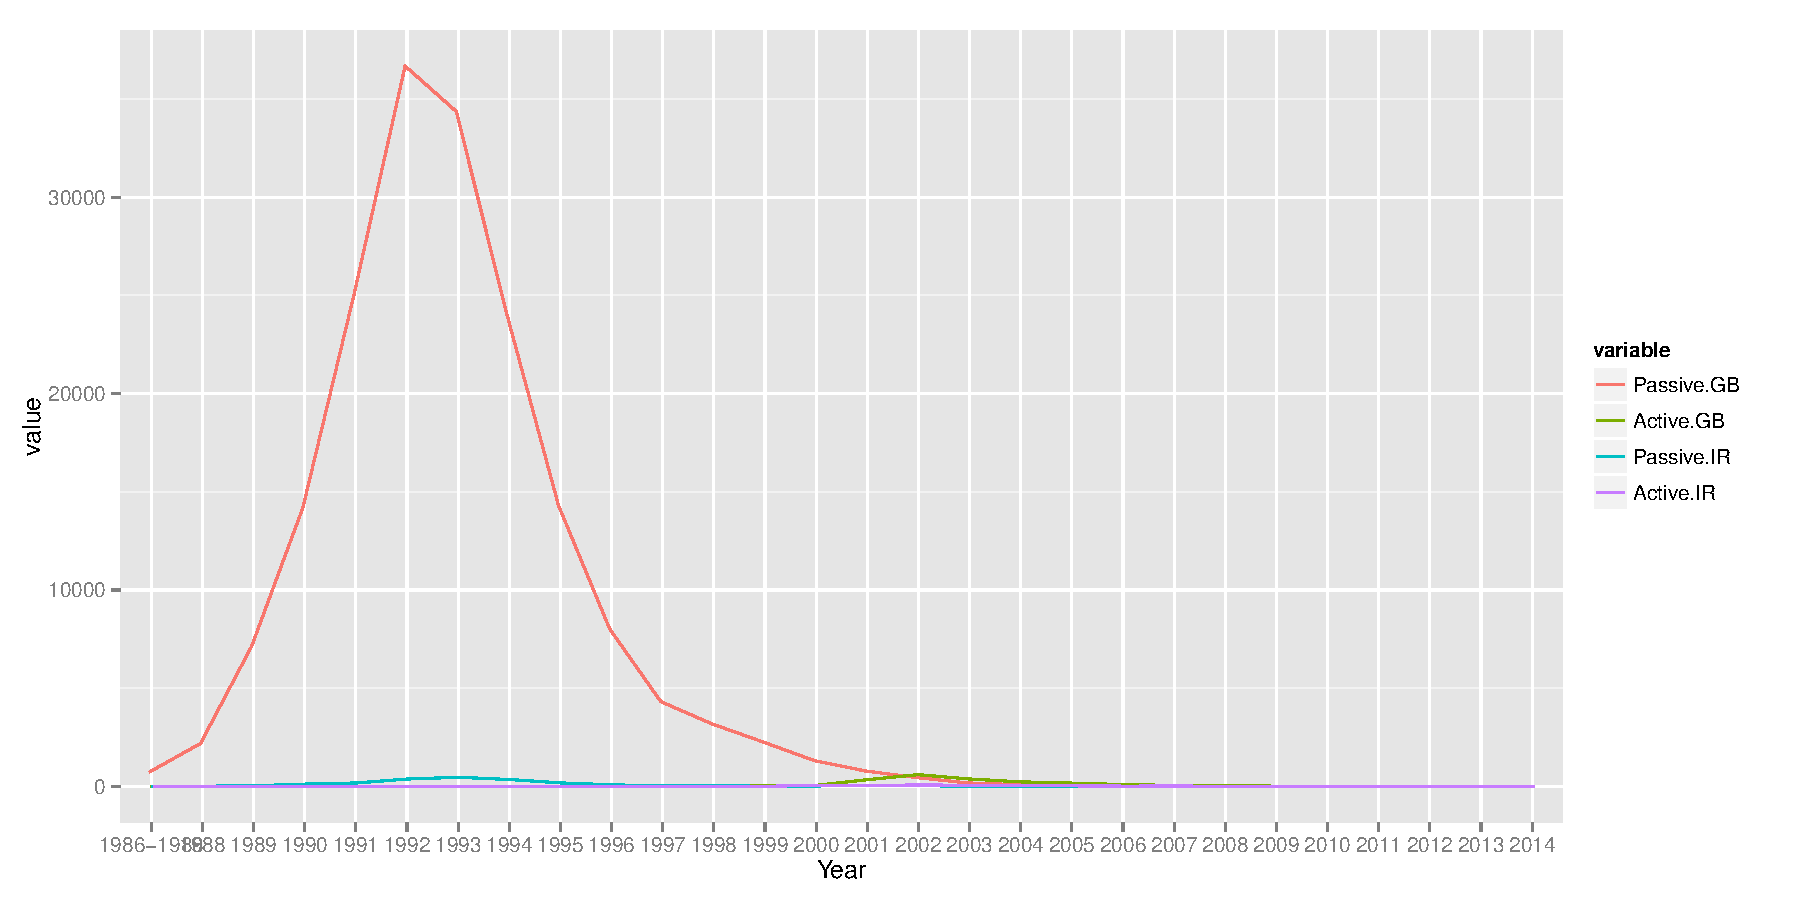
\includegraphics[width=\textwidth]{figure/subset} \caption[the general trend of BSE cases from 1987 to 2014 based on passive and active surveillance]{the general trend of BSE cases from 1987 to 2014 based on passive and active surveillance.\label{fig:subset}}
\end{figure}


\end{knitrout}


This plot shows the majority of data is from passive surveillance in great britain, and BSE cases were the most from 1989-1996.Now we can take a look at condition in great britain.

\subsection{Trend of passive surveillance in great britain}

\begin{knitrout}\footnotesize
\definecolor{shadecolor}{rgb}{0.969, 0.969, 0.969}\color{fgcolor}\begin{kframe}
\begin{alltt}
\hlstd{overall} \hlkwb{<-} \hlkwd{read.csv}\hlstd{(}\hlstr{"C:/Users/sding/Documents/GitHub/585xproject/OVERALL.csv"}\hlstd{)}
\hlstd{trend} \hlkwb{<-} \hlstd{overall[}\hlnum{1}\hlopt{:}\hlnum{28}\hlstd{, ]}
\hlstd{trend.det} \hlkwb{<-} \hlkwd{melt}\hlstd{(trend)}
\end{alltt}


{\ttfamily\noindent\itshape\color{messagecolor}{\#\# Using YEAR as id variables}}\begin{alltt}
\hlstd{pd} \hlkwb{<-} \hlkwd{position_dodge}\hlstd{(}\hlnum{0.1}\hlstd{)}
\hlstd{r} \hlkwb{<-} \hlkwd{ggplot}\hlstd{(}\hlkwc{data} \hlstd{= trend.det,} \hlkwd{aes}\hlstd{(}\hlkwc{x} \hlstd{= YEAR,} \hlkwc{y} \hlstd{= value,} \hlkwc{colour} \hlstd{= variable))} \hlopt{+}
    \hlkwd{geom_line}\hlstd{(}\hlkwc{position} \hlstd{= pd,} \hlkwd{aes}\hlstd{(}\hlkwc{group} \hlstd{= variable))}
\hlkwd{plot}\hlstd{(r)}
\end{alltt}


{\ttfamily\noindent\itshape\color{messagecolor}{\#\# ymax not defined: adjusting position using y instead}}\end{kframe}\begin{figure}[H]

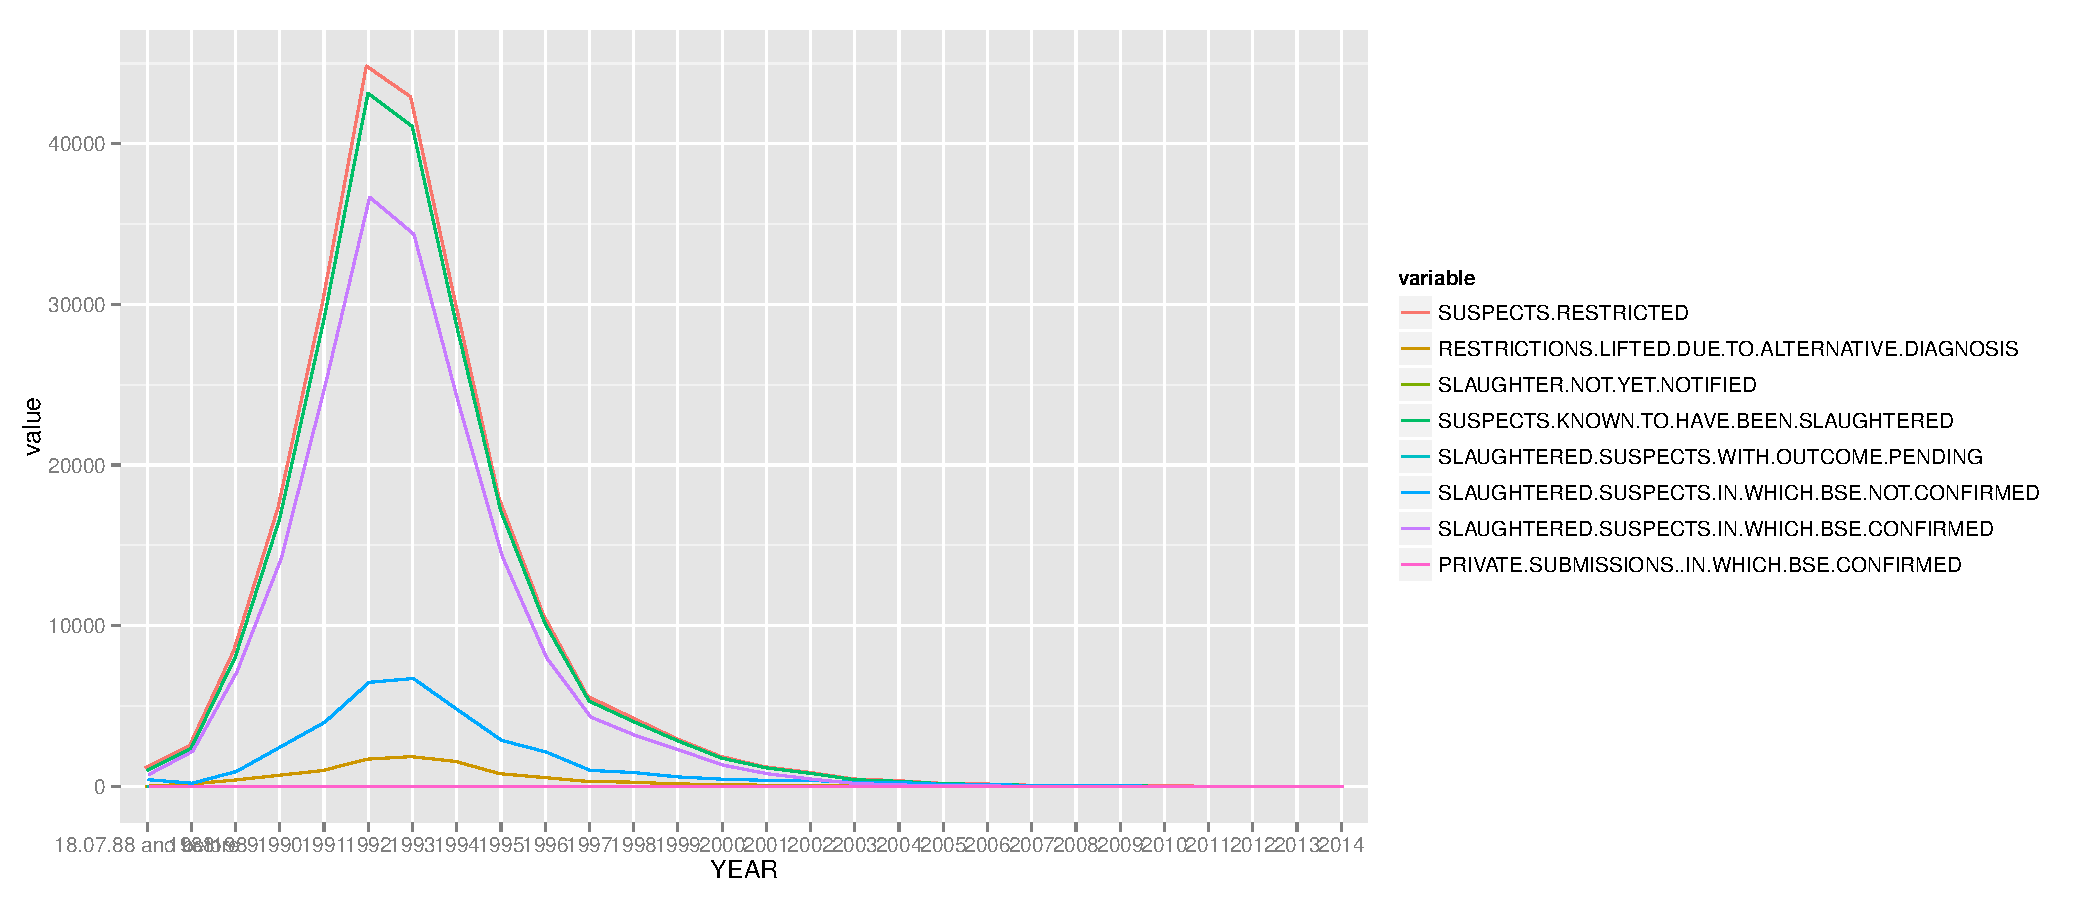
\includegraphics[width=\textwidth]{figure/GB} \caption[the trend of passive surveillance in great britain]{the trend of passive surveillance in great britain.\label{fig:GB}}
\end{figure}


\end{knitrout}


This plot shows the trend of restricted case and confirmed case. They all follow the similar curve, but the amplitude is different. The amount of suspected cases is a lot and almost all of those animals were slaughtered. Among them, the purple curve represents the actual confirmed cases.

\subsection{Cattle population over 24 months of ages and number of confirmed cases per million}
Since  the population of cattles were not contant during the time when people recorded the data, it is meaningful to take a look at the percentage of suspected of animals based on a time interval. Also, because of  a big moraility rate, the analysis can be focused on cattle with age older than 24 months. The x axis is the period when people took measurement, and the y axis is the amount of cattles confirmed with BSE disease.

\begin{knitrout}\footnotesize
\definecolor{shadecolor}{rgb}{0.969, 0.969, 0.969}\color{fgcolor}\begin{kframe}
\begin{alltt}
\hlkwd{library}\hlstd{(reshape)}
\hlkwd{library}\hlstd{(ggplot2)}
\hlkwd{library}\hlstd{(Mcow)}
\end{alltt}


{\ttfamily\noindent\itshape\color{messagecolor}{\#\# \\\#\# Attaching package: 'Mcow'\\\#\# \\\#\# The following object is masked from 'package:base':\\\#\# \\\#\#\ \ \ \  date}}\begin{alltt}
\hlstd{age24} \hlkwb{<-} \hlkwd{read.csv}\hlstd{(}\hlstr{"C:/Users/sding/Documents/GitHub/585xproject/millioncattle.csv"}\hlstd{)}
\hlstd{age24} \hlkwb{<-} \hlstd{age24[}\hlkwd{c}\hlstd{(}\hlnum{1}\hlopt{:}\hlnum{75}\hlstd{),} \hlopt{-}\hlkwd{c}\hlstd{(}\hlnum{5}\hlstd{,} \hlnum{8}\hlstd{)]}
\hlkwd{colnames}\hlstd{(age24)} \hlkwb{<-} \hlkwd{c}\hlstd{(}\hlstr{"start"}\hlstd{,} \hlstr{"end"}\hlstd{,} \hlstr{"million of cattles"}\hlstd{,} \hlstr{"# of case by date of confirmation"}\hlstd{,}
    \hlstr{"# of case by date of restriction"}\hlstd{,} \hlstr{"# per million by data of confirmation"}\hlstd{,}
    \hlstr{"# per million by date of restriction"}\hlstd{)}
\hlstd{age.sub} \hlkwb{<-} \hlstd{age24[}\hlopt{-}\hlnum{1}\hlstd{, ]}
\hlstd{age.sub}\hlopt{$}\hlstd{name} \hlkwb{<-} \hlnum{1}\hlopt{:}\hlnum{74}
\hlstd{age.sub[,} \hlnum{1}\hlstd{]} \hlkwb{<-} \hlkwd{date}\hlstd{(age.sub[,} \hlnum{1}\hlstd{])}
\hlstd{age.sub[,} \hlnum{2}\hlstd{]} \hlkwb{<-} \hlkwd{date}\hlstd{(age.sub[,} \hlnum{2}\hlstd{])}
\hlstd{age.sub}\hlopt{$}\hlstr{"# per million by data of confirmation"} \hlkwb{<-} \hlkwd{as.numeric}\hlstd{(}\hlkwd{as.character}\hlstd{(age.sub}\hlopt{$}\hlstr{"# per million by data of confirmation"}\hlstd{))}
\hlstd{mdfr} \hlkwb{<-} \hlkwd{melt}\hlstd{(age.sub,} \hlkwc{measure.vars} \hlstd{=} \hlkwd{c}\hlstd{(}\hlstr{"start"}\hlstd{,} \hlstr{"end"}\hlstd{))}
\hlstd{a} \hlkwb{<-} \hlkwd{ggplot}\hlstd{(mdfr,} \hlkwd{aes}\hlstd{(mdfr}\hlopt{$}\hlstd{value,} \hlkwd{as.factor}\hlstd{(mdfr}\hlopt{$}\hlstr{"million of cattles"}\hlstd{)))} \hlopt{+} \hlkwd{geom_line}\hlstd{(}\hlkwc{size} \hlstd{=} \hlnum{1}\hlstd{)} \hlopt{+}
    \hlkwd{xlab}\hlstd{(}\hlstr{"year"}\hlstd{)} \hlopt{+} \hlkwd{ylab}\hlstd{(}\hlstr{"million of cattles"}\hlstd{)} \hlopt{+} \hlkwd{theme_bw}\hlstd{()}
\hlkwd{plot}\hlstd{(a)}
\end{alltt}
\end{kframe}\begin{figure}[H]

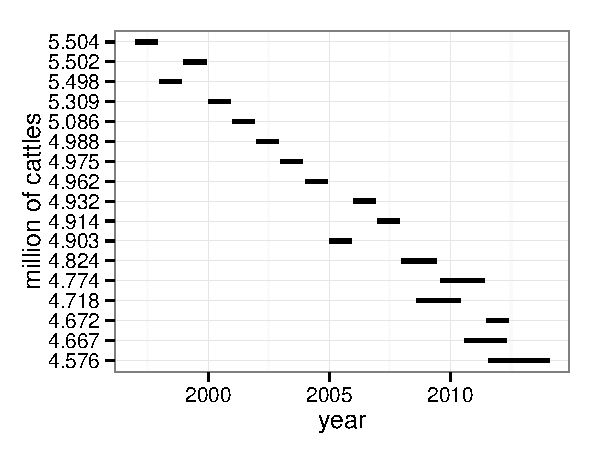
\includegraphics[width=\textwidth]{figure/r} \caption[Population of cattles]{Population of cattles.\label{fig:r}}
\end{figure}


\end{knitrout}

This plot indicates the population from 1987 to 2014 has been decreasing and the lowest level is in 2014, which might be under the influence of BSE disease. BSE caused the decrease of the demand of beef and this corresponds to the trend as shown in the plot.
\begin{knitrout}\footnotesize
\definecolor{shadecolor}{rgb}{0.969, 0.969, 0.969}\color{fgcolor}\begin{figure}[H]

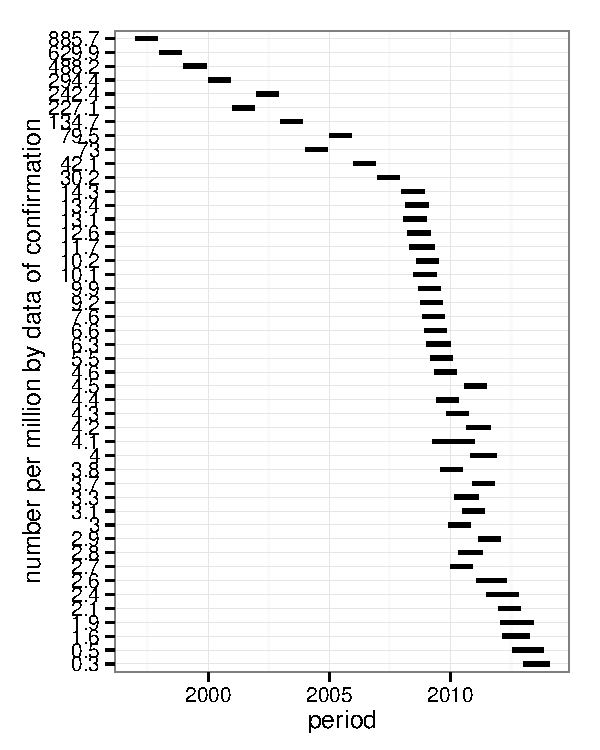
\includegraphics[width=\textwidth]{figure/percent} \caption[Number of confirmed BSE per million by date of confirmation]{Number of confirmed BSE per million by date of confirmation\label{fig:percent}}
\end{figure}


\end{knitrout}

With adequate control, from 2008 to 2014 the percentage of BSE cases has been decreasing dramatically. Compared to this, the period from 1987 to 2008, when the BSE was relativaly more serious, shows slower decreasing rate.

\subsection{Distribution of BSE in Great Britain}

\begin{knitrout}\footnotesize
\definecolor{shadecolor}{rgb}{0.969, 0.969, 0.969}\color{fgcolor}\begin{kframe}
\begin{alltt}
\hlkwd{library}\hlstd{(maptools)}
\end{alltt}


{\ttfamily\noindent\itshape\color{messagecolor}{\#\# Loading required package: sp\\\#\# Checking rgeos availability: FALSE\\\#\#\ \ 	Note: when rgeos is not available, polygon geometry 	computations in maptools depend on gpclib,\\\#\#\ \ 	which has a restricted licence. It is disabled by default;\\\#\#\ \ 	to enable gpclib, type gpclibPermit()}}\begin{alltt}
\hlkwd{library}\hlstd{(Mcow)}
\hlstd{city} \hlkwb{<-} \hlkwd{read.csv}\hlstd{(}\hlstr{"C:/Users/sding/Documents/GitHub/585xproject/city.csv"}\hlstd{)}
\hlstd{uk} \hlkwb{<-} \hlkwd{readShapeSpatial}\hlstd{(}\hlstr{"C:/Users/sding/Documents/GitHub/585xproject/uk/map.shp"}\hlstd{)}
\hlstd{xxx} \hlkwb{<-} \hlkwd{thinnedSpatialPoly}\hlstd{(}\hlkwd{as}\hlstd{(uk,} \hlstr{"SpatialPolygons"}\hlstd{),} \hlkwc{tolerance} \hlstd{=} \hlnum{0.1}\hlstd{,} \hlkwc{minarea} \hlstd{=} \hlnum{0.001}\hlstd{,}
    \hlkwc{topologyPreserve} \hlstd{=} \hlnum{TRUE}\hlstd{)}
\hlstd{oz} \hlkwb{<-} \hlkwd{extractPolygons}\hlstd{(xxx)}
\hlcom{# ggplot(oz, aes(x = x, y = y, group = group)) +}
\hlcom{# geom_polygon(colour='black', fill='white')}
\hlstd{uk}\hlopt{@}\hlkwc{data}\hlopt{$}\hlstd{MM_UID} \hlkwb{<-} \hlnum{1}\hlopt{:}\hlnum{192}
\hlstd{oz.new} \hlkwb{<-} \hlkwd{merge}\hlstd{(oz, uk}\hlopt{@}\hlkwc{data}\hlstd{,} \hlkwc{by.x} \hlstd{=} \hlstr{"region"}\hlstd{,} \hlkwc{by.y} \hlstd{=} \hlstr{"MM_UID"}\hlstd{)}
\hlcom{# Clean the data}
\hlstd{city}\hlopt{$}\hlstd{COUNTY} \hlkwb{<-} \hlkwd{gsub}\hlstd{(}\hlstr{"&"}\hlstd{,} \hlstr{"and"}\hlstd{, city}\hlopt{$}\hlstd{COUNTY)}
\hlstd{city}\hlopt{$}\hlstd{COUNTY[city}\hlopt{$}\hlstd{COUNTY} \hlopt{==} \hlstr{"Ayrshire"}\hlstd{]} \hlkwb{<-} \hlstr{"South Ayrshire"}
\hlstd{city}\hlopt{$}\hlstd{COUNTY[city}\hlopt{$}\hlstd{COUNTY} \hlopt{==} \hlstr{"Cornwall and Isles of Scilly"}\hlstd{]} \hlkwb{<-} \hlstr{"Cornwall"}
\hlstd{city}\hlopt{$}\hlstd{COUNTY[city}\hlopt{$}\hlstd{COUNTY} \hlopt{==} \hlstr{"East Riding and Northern Lincolnshire"}\hlstd{]} \hlkwb{<-} \hlstr{"North Lincolnshire"}
\hlstd{city}\hlopt{$}\hlstd{COUNTY[city}\hlopt{$}\hlstd{COUNTY} \hlopt{==} \hlstr{"Eileanan an lar"}\hlstd{]} \hlkwb{<-} \hlstr{"Eilean Siar"}
\hlstd{city}\hlopt{$}\hlstd{COUNTY[city}\hlopt{$}\hlstd{COUNTY} \hlopt{==} \hlstr{"Greater London"}\hlstd{]} \hlkwb{<-} \hlstr{"London"}
\hlstd{city}\hlopt{$}\hlstd{COUNTY[city}\hlopt{$}\hlstd{COUNTY} \hlopt{==} \hlstr{"Greater Manchester"}\hlstd{]} \hlkwb{<-} \hlstr{"Manchester"}
\hlstd{city}\hlopt{$}\hlstd{COUNTY[city}\hlopt{$}\hlstd{COUNTY} \hlopt{==} \hlstr{"Gloucestershire excl South"}\hlstd{]} \hlkwb{<-} \hlstr{"South Gloucestershire"}
\hlstd{city}\hlopt{$}\hlstd{COUNTY[city}\hlopt{$}\hlstd{COUNTY} \hlopt{==} \hlstr{"Leicestershire and Rutland"}\hlstd{]} \hlkwb{<-} \hlstr{"Leicestershire"}
\hlstd{city}\hlopt{$}\hlstd{COUNTY[city}\hlopt{$}\hlstd{COUNTY} \hlopt{==} \hlstr{"Lincolnshire excl North"}\hlstd{]} \hlkwb{<-} \hlstr{"North Lincolnshire"}
\hlstd{city}\hlopt{$}\hlstd{COUNTY[city}\hlopt{$}\hlstd{COUNTY} \hlopt{==} \hlstr{"North-East Scotland"}\hlstd{]} \hlkwb{<-} \hlstr{"Arberdeen"}
\hlstd{city}\hlopt{$}\hlstd{COUNTY[city}\hlopt{$}\hlstd{COUNTY} \hlopt{==} \hlstr{"North-East Wales"}\hlstd{]} \hlkwb{<-} \hlstr{"Herefordnshire"}
\hlstd{city}\hlopt{$}\hlstd{COUNTY[city}\hlopt{$}\hlstd{COUNTY} \hlopt{==} \hlstr{"North-West Wales"}\hlstd{]} \hlkwb{<-} \hlstr{"Ceredigion"}
\hlstd{city}\hlopt{$}\hlstd{COUNTY[city}\hlopt{$}\hlstd{COUNTY} \hlopt{==} \hlstr{"Northern Somerset and South Glouceste"}\hlstd{]} \hlkwb{<-} \hlstr{"Northern Somerset"}
\hlstd{city}\hlopt{$}\hlstd{COUNTY[city}\hlopt{$}\hlstd{COUNTY} \hlopt{==} \hlstr{"Somerset excl North"}\hlstd{]} \hlkwb{<-} \hlstr{"North Somerset"}
\hlstd{city}\hlopt{$}\hlstd{COUNTY[city}\hlopt{$}\hlstd{COUNTY} \hlopt{==} \hlstr{"South Wales"}\hlstd{]} \hlkwb{<-} \hlstr{"Cardiff"}
\hlkwd{colnames}\hlstd{(city)} \hlkwb{<-} \hlkwd{c}\hlstd{(}\hlstr{"region"}\hlstd{,} \hlstr{"farms"}\hlstd{,} \hlstr{"cases"}\hlstd{)}
\hlstd{oz.subset} \hlkwb{<-} \hlstd{oz.new[,} \hlkwd{c}\hlstd{(}\hlnum{2}\hlopt{:}\hlnum{5}\hlstd{,} \hlnum{7}\hlstd{,} \hlnum{8}\hlstd{,} \hlnum{9}\hlstd{)]}
\hlkwd{colnames}\hlstd{(oz.subset)} \hlkwb{<-} \hlkwd{c}\hlstd{(}\hlstr{"x"}\hlstd{,} \hlstr{"y"}\hlstd{,} \hlstr{"order"}\hlstd{,} \hlstr{"group"}\hlstd{,} \hlstr{"area"}\hlstd{,} \hlstr{"region"}\hlstd{,} \hlstr{"division"}\hlstd{)}
\hlcom{# merge two files}
\hlstd{distribution} \hlkwb{<-} \hlkwd{merge}\hlstd{(oz.subset, city,} \hlkwc{by} \hlstd{=} \hlstr{"region"}\hlstd{)}
\hlcom{# distribution of farms and BSE cases}
\hlstd{distribution}\hlopt{$}\hlstd{cases} \hlkwb{<-} \hlkwd{as.numeric}\hlstd{(distribution}\hlopt{$}\hlstd{cases)}
\hlstd{a} \hlkwb{<-} \hlkwd{ggplot}\hlstd{()} \hlopt{+} \hlkwd{geom_polygon}\hlstd{(}\hlkwc{data} \hlstd{= oz.new,} \hlkwd{aes}\hlstd{(}\hlkwc{x} \hlstd{= x,} \hlkwc{y} \hlstd{= y,} \hlkwc{order} \hlstd{= order,}
    \hlkwc{group} \hlstd{= group))} \hlopt{+} \hlkwd{geom_polygon}\hlstd{(}\hlkwc{data} \hlstd{= distribution,} \hlkwd{aes}\hlstd{(}\hlkwc{x} \hlstd{= x,} \hlkwc{y} \hlstd{= y,} \hlkwc{order} \hlstd{= order,}
    \hlkwc{group} \hlstd{= group,} \hlkwc{fill} \hlstd{= distribution}\hlopt{$}\hlstd{cases))}
\hlkwd{plot}\hlstd{(a)}
\end{alltt}
\end{kframe}\begin{figure}[H]

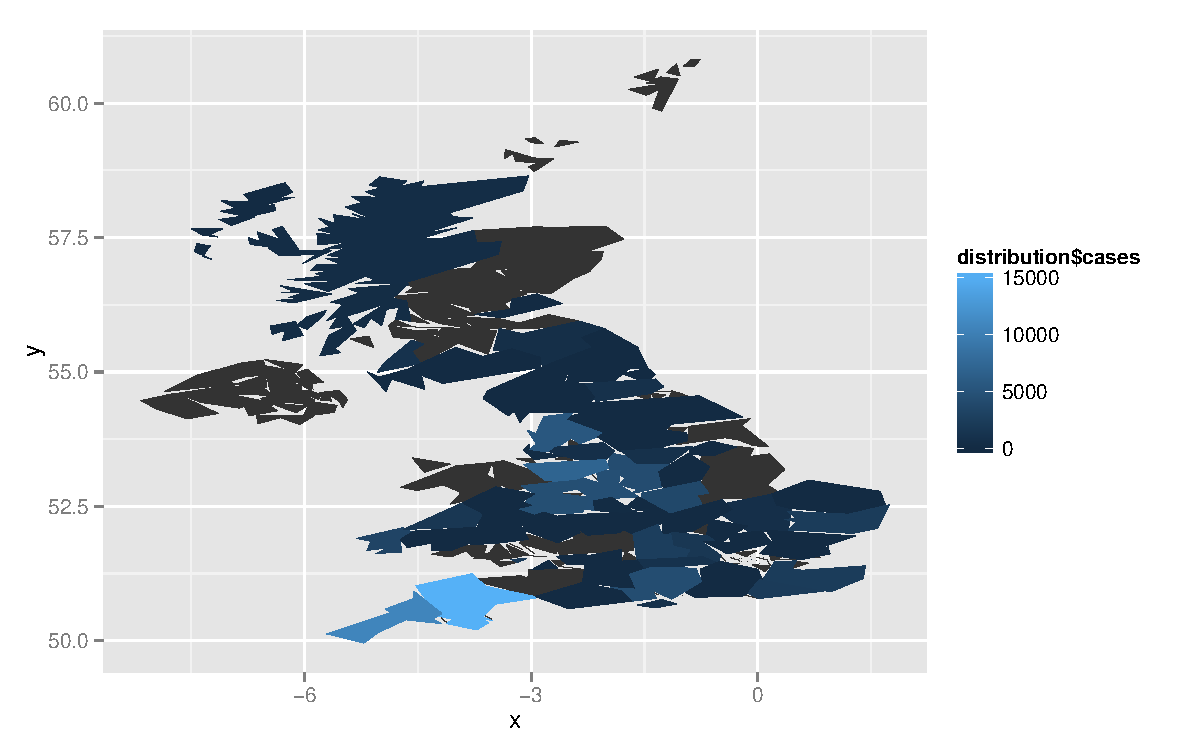
\includegraphics[width=\textwidth]{figure/map} \caption[Distribution of BSE cases in Great Britain]{Distribution of BSE cases in Great Britain\label{fig:map}}
\end{figure}


\end{knitrout}


\begin{knitrout}\footnotesize
\definecolor{shadecolor}{rgb}{0.969, 0.969, 0.969}\color{fgcolor}\begin{figure}[H]

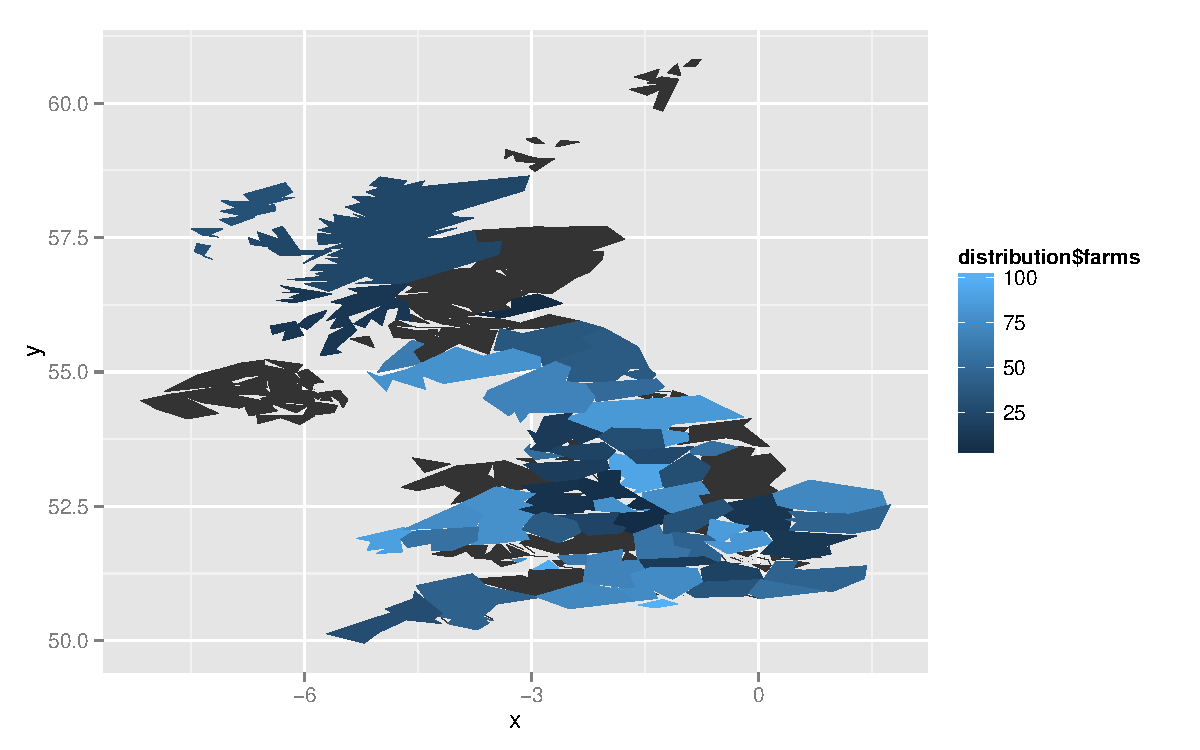
\includegraphics[width=\textwidth]{figure/farm} \caption[Distribution of farms where BSE have been found in Great Britain]{Distribution of farms where BSE have been found in Great Britain\label{fig:farm}}
\end{figure}


\end{knitrout}

The color gradient indicates the distribution of BSE cases and farms where BSE cases have been found.

\subsection{Percent reduction of BSE cases in each year}
\begin{knitrout}\footnotesize
\definecolor{shadecolor}{rgb}{0.969, 0.969, 0.969}\color{fgcolor}\begin{kframe}
\begin{alltt}
\hlstd{red} \hlkwb{<-} \hlstd{trend[,} \hlkwd{c}\hlstd{(}\hlnum{1}\hlstd{,} \hlnum{2}\hlstd{,} \hlnum{8}\hlstd{)]}
\hlstd{red}\hlopt{$}\hlstr{"percent reduction year on year(suspected)"} \hlkwb{<-} \hlnum{NA}
\hlstd{red}\hlopt{$}\hlstr{"percent reduction year on year(confirmed)"} \hlkwb{<-} \hlnum{NA}
\hlstd{i} \hlkwb{<-} \hlnum{NA}
\hlstd{j} \hlkwb{<-} \hlnum{NA}
\hlstd{per} \hlkwb{<-} \hlnum{NA}
\hlstd{red[}\hlnum{1}\hlopt{:}\hlnum{28}\hlstd{,} \hlnum{2}\hlopt{:}\hlnum{3}\hlstd{]} \hlkwb{<-} \hlkwd{as.matrix}\hlstd{(}\hlkwd{sapply}\hlstd{(red[}\hlnum{1}\hlopt{:}\hlnum{28}\hlstd{,} \hlnum{2}\hlopt{:}\hlnum{3}\hlstd{], as.numeric))}
\hlstd{percent} \hlkwb{<-} \hlkwa{function}\hlstd{(}\hlkwc{x}\hlstd{,} \hlkwc{digits} \hlstd{=} \hlnum{2}\hlstd{,} \hlkwc{format} \hlstd{=} \hlstr{"f"}\hlstd{,} \hlkwc{...}\hlstd{) \{}
    \hlkwd{paste}\hlstd{(}\hlkwd{formatC}\hlstd{(}\hlnum{100} \hlopt{*} \hlstd{x,} \hlkwc{format} \hlstd{= format,} \hlkwc{digits} \hlstd{= digits, ...),} \hlstr{"%"}\hlstd{,} \hlkwc{sep} \hlstd{=} \hlstr{""}\hlstd{)}
\hlstd{\}}

\hlkwa{for} \hlstd{(i} \hlkwa{in} \hlnum{3}\hlopt{:}\hlstd{(}\hlkwd{length}\hlstd{(red}\hlopt{$}\hlstd{SUSPECTS.RESTRICTED))) \{}
    \hlstd{red}\hlopt{$}\hlstr{"percent reduction year on year(suspected)"}\hlstd{[i]} \hlkwb{<-} \hlkwd{as.numeric}\hlstd{((}\hlopt{-}\hlstd{red}\hlopt{$}\hlstd{SUSPECTS.RESTRICTED[i} \hlopt{-}
        \hlnum{1}\hlstd{]} \hlopt{+} \hlstd{red}\hlopt{$}\hlstd{SUSPECTS.RESTRICTED[i])}\hlopt{/}\hlstd{red}\hlopt{$}\hlstd{SUSPECTS.RESTRICTED[i} \hlopt{-} \hlnum{1}\hlstd{])}
    \hlstd{red}\hlopt{$}\hlstr{"percent reduction year on year(confirmed)"}\hlstd{[i]} \hlkwb{<-} \hlkwd{as.numeric}\hlstd{((}\hlopt{-}\hlstd{red}\hlopt{$}\hlstd{SLAUGHTERED.SUSPECTS.IN.WHICH.BSE.CONFIRMED[i} \hlopt{-}
        \hlnum{1}\hlstd{]} \hlopt{+} \hlstd{red}\hlopt{$}\hlstd{SLAUGHTERED.SUSPECTS.IN.WHICH.BSE.CONFIRMED[i])}\hlopt{/}\hlstd{red}\hlopt{$}\hlstd{SLAUGHTERED.SUSPECTS.IN.WHICH.BSE.CONFIRMED[i} \hlopt{-}
        \hlnum{1}\hlstd{])}
    \hlkwa{if} \hlstd{(red}\hlopt{$}\hlstd{SLAUGHTERED.SUSPECTS.IN.WHICH.BSE.CONFIRMED[i} \hlopt{-} \hlnum{1}\hlstd{]} \hlopt{==} \hlnum{0}\hlstd{) \{}
        \hlstd{red}\hlopt{$}\hlstr{"percent reduction year on year(confirmed)"}\hlstd{[i]} \hlkwb{<-} \hlnum{0}
    \hlstd{\}}
\hlstd{\}}

\hlstd{red.melt} \hlkwb{<-} \hlkwd{melt}\hlstd{(red[,} \hlkwd{c}\hlstd{(}\hlnum{1}\hlstd{,} \hlnum{4}\hlstd{,} \hlnum{5}\hlstd{)],} \hlkwc{id} \hlstd{=} \hlkwd{c}\hlstd{(}\hlstr{"YEAR"}\hlstd{))}
\hlstd{red.melt}\hlopt{$}\hlstd{value} \hlkwb{<-} \hlkwd{as.numeric}\hlstd{(red.melt}\hlopt{$}\hlstd{value)}
\hlstd{red.melt}\hlopt{$}\hlstd{value[}\hlkwd{is.na}\hlstd{(red.melt}\hlopt{$}\hlstd{value)]} \hlkwb{<-} \hlnum{0}
\hlstd{pd} \hlkwb{<-} \hlkwd{position_dodge}\hlstd{(}\hlnum{0.1}\hlstd{)}
\hlstd{a} \hlkwb{<-} \hlkwd{ggplot}\hlstd{(}\hlkwc{data} \hlstd{= red.melt,} \hlkwd{aes}\hlstd{(}\hlkwc{x} \hlstd{= YEAR,} \hlkwc{y} \hlstd{= value,} \hlkwc{colour} \hlstd{= variable))} \hlopt{+}
    \hlkwd{geom_line}\hlstd{(}\hlkwc{position} \hlstd{= pd,} \hlkwd{aes}\hlstd{(}\hlkwc{group} \hlstd{= variable))}
\hlkwd{plot}\hlstd{(a)}
\end{alltt}


{\ttfamily\noindent\itshape\color{messagecolor}{\#\# ymax not defined: adjusting position using y instead}}\end{kframe}\begin{figure}[H]

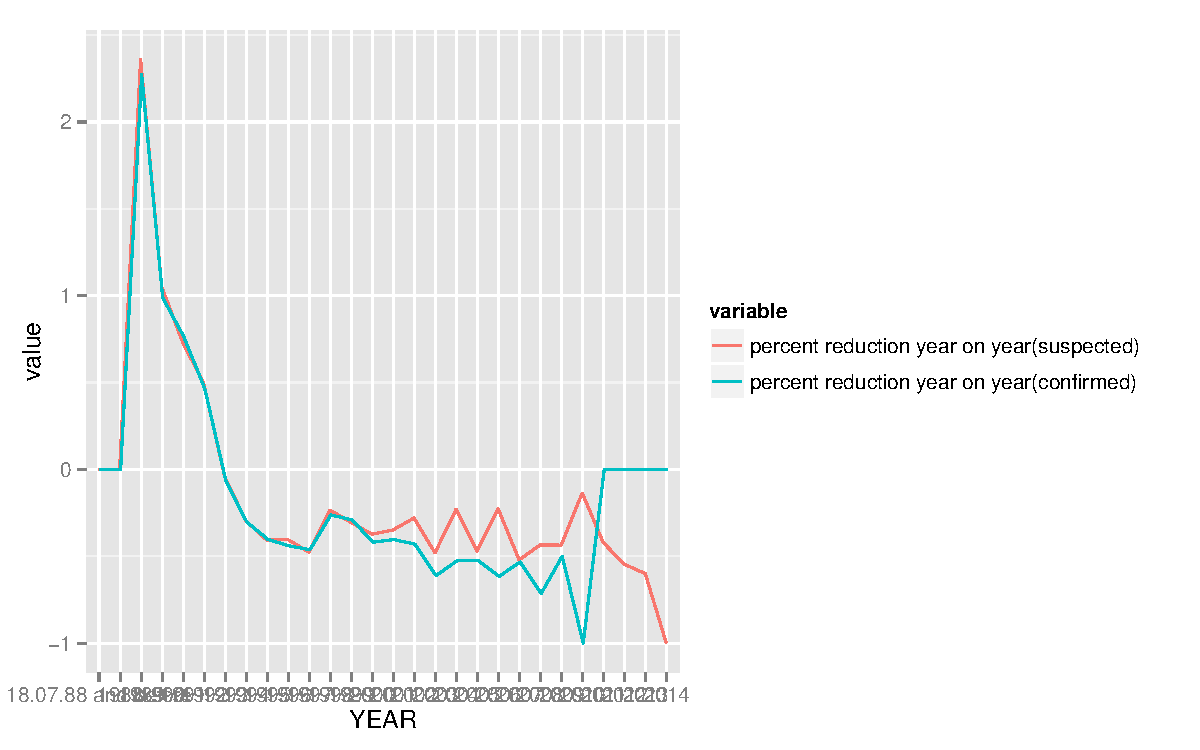
\includegraphics[width=\textwidth]{figure/reduction} \caption[Percentage reduction]{Percentage reduction\label{fig:reduction}}
\end{figure}


\end{knitrout}

This plot shows the percentage reduction of confirmed and suspected cases year on year.

\subsection{The trend of confirmed BSE cases of different age in great britain}
\begin{knitrout}\footnotesize
\definecolor{shadecolor}{rgb}{0.969, 0.969, 0.969}\color{fgcolor}\begin{kframe}
\begin{alltt}
\hlstd{age} \hlkwb{<-} \hlkwd{read.csv}\hlstd{(}\hlstr{"C:/Users/sding/Documents/GitHub/585xproject/age.gb.csv"}\hlstd{)}
\hlstd{age} \hlkwb{<-} \hlstd{age[}\hlopt{-}\hlnum{1}\hlstd{,} \hlopt{-}\hlnum{2}\hlstd{]}
\hlstd{age}\hlopt{$}\hlstr{"Birth Period"} \hlkwb{<-} \hlnum{1982}\hlopt{:}\hlnum{2006}
\end{alltt}


{\ttfamily\noindent\bfseries\color{errorcolor}{\#\# Error: replacement has 25 rows, data has 27}}\begin{alltt}
\hlkwd{colnames}\hlstd{(age)} \hlkwb{<-} \hlkwd{c}\hlstd{(}\hlstr{"Birth Period"}\hlstd{,} \hlstr{"1 year old"}\hlstd{,} \hlstr{"2 year old"}\hlstd{,} \hlstr{"3 year old"}\hlstd{,}
    \hlstr{"4 year old"}\hlstd{,} \hlstr{"5 year old"}\hlstd{,} \hlstr{"6 year old"}\hlstd{,} \hlstr{"7 year old"}\hlstd{,} \hlstr{"8 year old"}\hlstd{,} \hlstr{"9 year old"}\hlstd{,}
    \hlstr{"10 year old"}\hlstd{)}
\hlstd{age.melt} \hlkwb{<-} \hlkwd{melt}\hlstd{(age,} \hlkwc{id} \hlstd{=} \hlstr{"Birth Period"}\hlstd{)}
\hlstd{age.melt}\hlopt{$}\hlstd{value} \hlkwb{<-} \hlkwd{as.numeric}\hlstd{(age.melt}\hlopt{$}\hlstd{value)}
\hlstd{age.melt}\hlopt{$}\hlstr{"Birth Period"} \hlkwb{<-} \hlkwd{as.numeric}\hlstd{(age.melt}\hlopt{$}\hlstr{"Birth Period"}\hlstd{)}
\hlstd{age.melt}\hlopt{$}\hlstd{variable} \hlkwb{<-} \hlkwd{as.factor}\hlstd{(age.melt}\hlopt{$}\hlstd{variable)}

\hlstd{pd} \hlkwb{<-} \hlkwd{position_dodge}\hlstd{(}\hlnum{0.1}\hlstd{)}
\hlstd{a} \hlkwb{<-} \hlkwd{ggplot}\hlstd{(}\hlkwc{data} \hlstd{= age.melt,} \hlkwd{aes}\hlstd{(}\hlkwc{x} \hlstd{= age.melt}\hlopt{$}\hlstr{"Birth Period"}\hlstd{,} \hlkwc{y} \hlstd{= value,} \hlkwc{colour} \hlstd{= variable))} \hlopt{+}
    \hlkwd{geom_line}\hlstd{(}\hlkwc{position} \hlstd{= pd,} \hlkwd{aes}\hlstd{(}\hlkwc{group} \hlstd{= variable))}
\hlkwd{plot}\hlstd{(a)}
\end{alltt}


{\ttfamily\noindent\itshape\color{messagecolor}{\#\# ymax not defined: adjusting position using y instead}}\end{kframe}\begin{figure}[H]

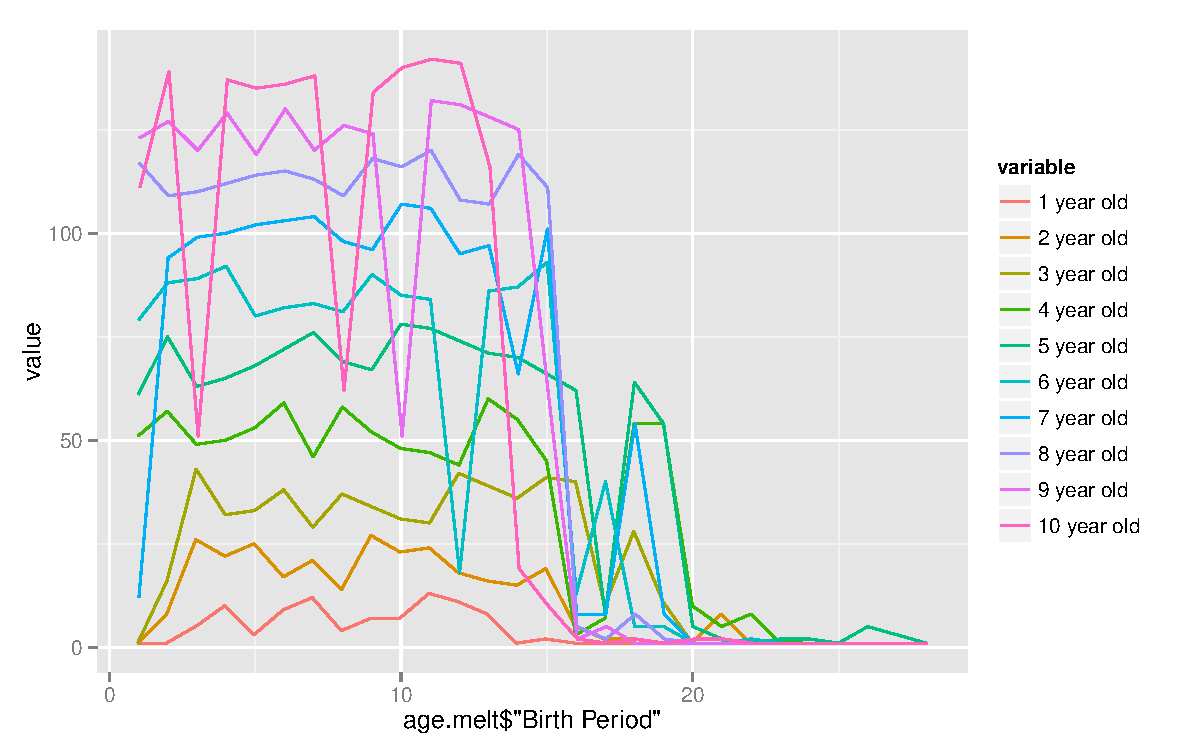
\includegraphics[width=\textwidth]{figure/age} \caption[confirmed BSE cases of different age]{confirmed BSE cases of different age\label{fig:age}}
\end{figure}


\end{knitrout}


If we set age as a factor, age of the animals seems to be proportional to number of cases. 

\subsection{The distribution of BSE cases in Great Britain from 2013 to 2014}
\begin{knitrout}\footnotesize
\definecolor{shadecolor}{rgb}{0.969, 0.969, 0.969}\color{fgcolor}\begin{kframe}
\begin{alltt}
\hlstd{recent} \hlkwb{<-} \hlkwd{read.csv}\hlstd{(}\hlstr{"C:/Users/sding/Documents/GitHub/585xproject/recent.csv"}\hlstd{)}
\hlstd{a} \hlkwb{<-} \hlstd{recent[}\hlopt{-}\hlnum{1}\hlstd{,} \hlkwd{c}\hlstd{(}\hlnum{1}\hlstd{,} \hlnum{2}\hlstd{,} \hlnum{3}\hlstd{,} \hlnum{4}\hlstd{)]}
\hlstd{recent[,} \hlkwd{c}\hlstd{(}\hlnum{2}\hlstd{,} \hlnum{3}\hlstd{,} \hlnum{4}\hlstd{)]} \hlkwb{<-} \hlkwd{as.matrix}\hlstd{(}\hlkwd{sapply}\hlstd{(recent[,} \hlkwd{c}\hlstd{(}\hlnum{2}\hlstd{,} \hlnum{3}\hlstd{,} \hlnum{4}\hlstd{)], as.numeric))}
\hlstd{a}\hlopt{$}\hlstd{cases} \hlkwb{<-} \hlkwd{rowSums}\hlstd{(recent[}\hlopt{-}\hlnum{1}\hlstd{,} \hlkwd{c}\hlstd{(}\hlnum{2}\hlstd{,} \hlnum{3}\hlstd{,} \hlnum{4}\hlstd{)])}
\hlstd{a}\hlopt{$}\hlstd{County} \hlkwb{<-} \hlkwd{gsub}\hlstd{(}\hlstr{"&"}\hlstd{,} \hlstr{"and"}\hlstd{, a}\hlopt{$}\hlstd{County)}
\hlstd{a} \hlkwb{<-} \hlstd{a[,} \hlopt{-}\hlkwd{c}\hlstd{(}\hlnum{2}\hlstd{,} \hlnum{3}\hlstd{,} \hlnum{4}\hlstd{)]}
\hlstd{a}\hlopt{$}\hlstd{County[a}\hlopt{$}\hlstd{County} \hlopt{==} \hlstr{"North-West Wales"}\hlstd{]} \hlkwb{<-} \hlstr{"Ceredigion"}
\hlkwd{colnames}\hlstd{(a)} \hlkwb{<-} \hlkwd{c}\hlstd{(}\hlstr{"region"}\hlstd{,} \hlstr{"cases"}\hlstd{)}

\hlstd{rec.dis} \hlkwb{<-} \hlkwd{merge}\hlstd{(oz.subset, a,} \hlkwc{by} \hlstd{=} \hlstr{"region"}\hlstd{)}
\hlstd{rec.dis}\hlopt{$}\hlstd{cases} \hlkwb{<-} \hlkwd{as.numeric}\hlstd{(rec.dis}\hlopt{$}\hlstd{cases)}
\hlstd{a} \hlkwb{<-} \hlkwd{ggplot}\hlstd{()} \hlopt{+} \hlkwd{geom_polygon}\hlstd{(}\hlkwc{data} \hlstd{= oz.subset,} \hlkwd{aes}\hlstd{(}\hlkwc{x} \hlstd{= x,} \hlkwc{y} \hlstd{= y,} \hlkwc{order} \hlstd{= order,}
    \hlkwc{group} \hlstd{= group))} \hlopt{+} \hlkwd{geom_polygon}\hlstd{(}\hlkwc{data} \hlstd{= rec.dis,} \hlkwd{aes}\hlstd{(}\hlkwc{x} \hlstd{= x,} \hlkwc{y} \hlstd{= y,} \hlkwc{order} \hlstd{= order,}
    \hlkwc{group} \hlstd{= group,} \hlkwc{fill} \hlstd{= rec.dis}\hlopt{$}\hlstd{cases))}
\hlkwd{plot}\hlstd{(a)}
\end{alltt}
\end{kframe}\begin{figure}[H]

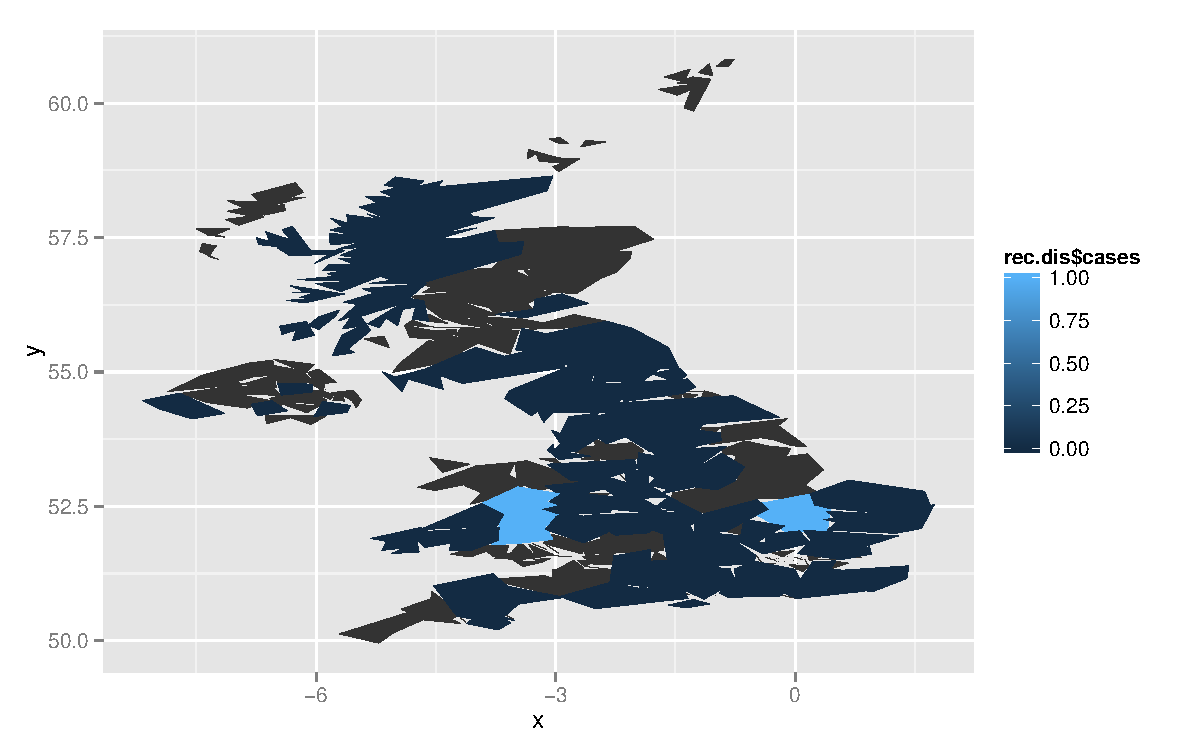
\includegraphics[width=\textwidth]{figure/recent} \caption[The distribution of BSE cases in Great Britain from 2013 to 2014]{The distribution of BSE cases in Great Britain from 2013 to 2014\label{fig:recent}}
\end{figure}


\end{knitrout}

Even though BSE is no longer active in the UK, there are still cases appeared in recent years. Since prion disease is hard to diagnose and it spread easily through food contamination, attention is still required to monitor the development of BSE.

\section{Shiny App for Raman analysis}

library(shiny)
runGist(11195851)

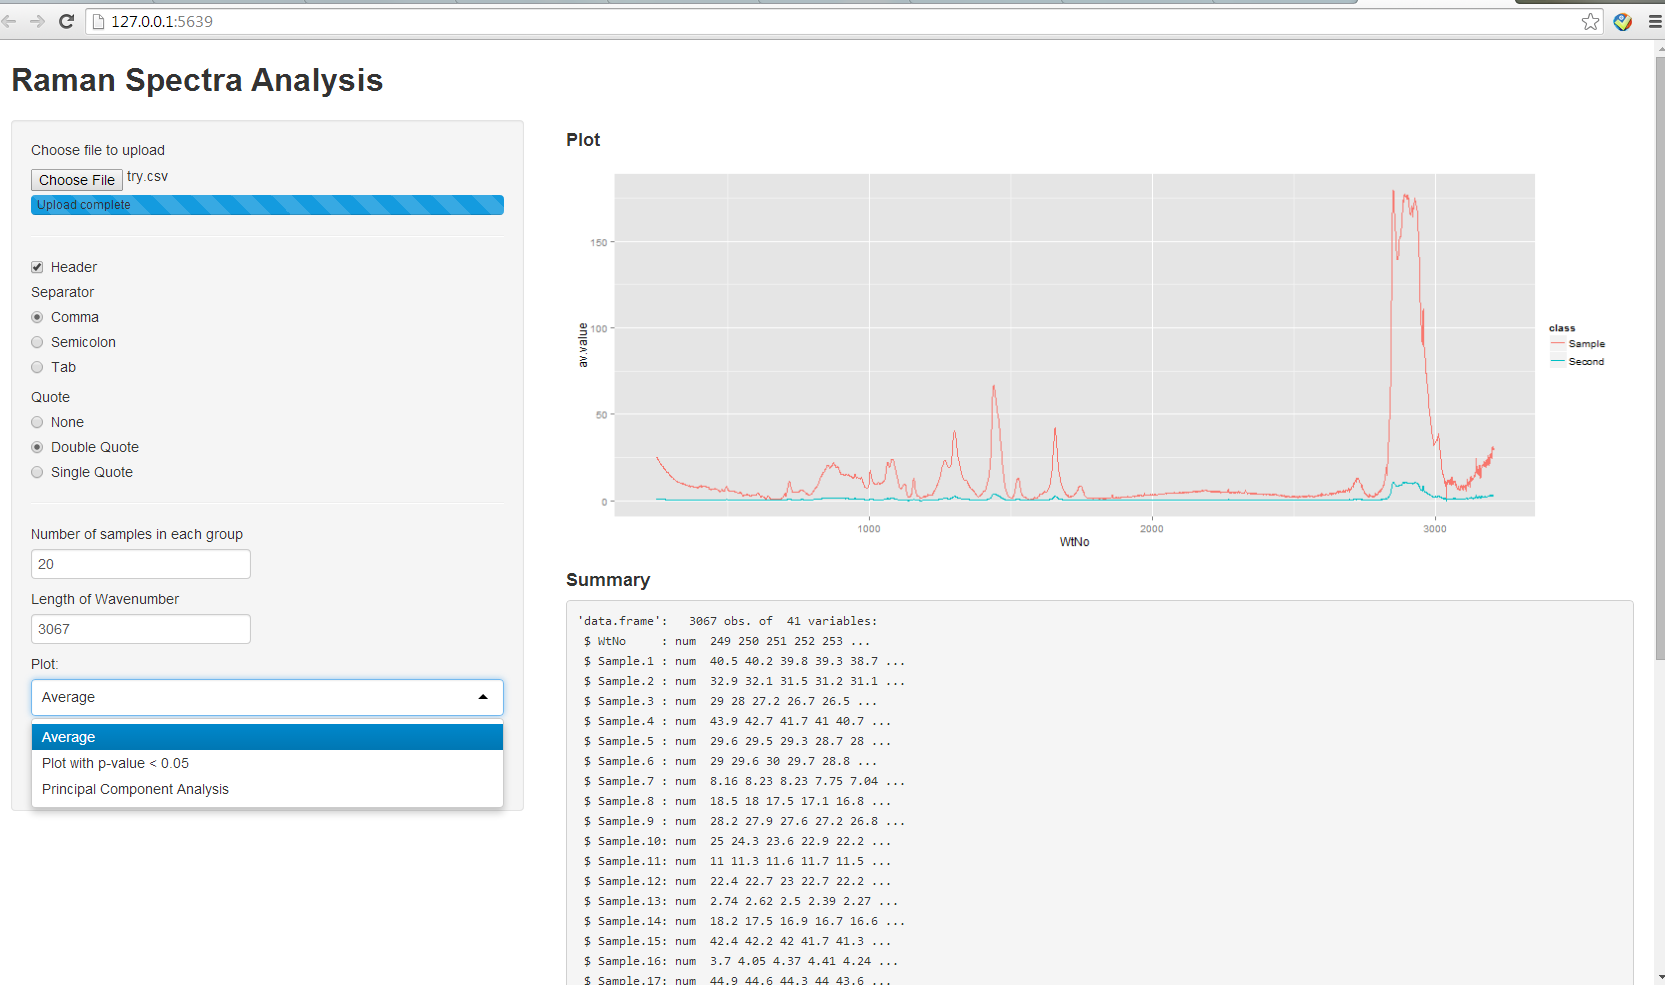
\includegraphics[width=\textwidth]{shiny.png}
The screenshot above is the shiny app I built for Raman spectra analysis. Data is uploaded as required format and based on user's preferance, the desired plot will be displayed in the main panel. Additionally, the result can be downloaded from the buttion on the left. However, uploaded data need to be corrected by polynomial baseline correction, smoothing and normalization.
 
\section{Mcow package}
The packages I built for this project is consisted of 4 functions: data,extractPolygons(the function in class),percent and percentage_reduction. This is not quite complete and some modifications need to be made.

date: This function to reformat the date in the given dataset
extractPolygons: The function to extract polygons
percent: The function to format data into percentage format
percent_reduction: This function to calculate percent reduction year on year
                        
\section{Discussion and Conclusion}

From this analysis,BSE cases have been decreasing dramatically during the past decade, however, there are still BSE existing and more prion diseases like scrapie and CJDs appear, which threaten human and animal health. Since prion caused disease is very hard to diagnose, with the application of Raman Spectroscopy, people can dectect the protein transformation at a earlier stage, which is beneficial for diease control, as well leading to a better medical treatment.

\end{document}
